\documentclass[15pt,a5paper,reqno]{article}
\usepackage{hyperref}
\usepackage[warn]{mathtext}
\usepackage[utf8]{inputenc}
\usepackage[T2A]{fontenc}
\usepackage[russian]{babel}
\usepackage{amssymb, amsmath, multicol}
\usepackage{graphicx}
\usepackage[shortcuts,cyremdash]{extdash}
\usepackage{wrapfig}
\usepackage{floatflt}
\usepackage{lipsum}
\usepackage{verbatim}
\usepackage{concmath}
\usepackage{euler}
\usepackage{xcolor}
\usepackage{etoolbox}
\usepackage{fancyhdr}
\usepackage{subfiles}
\usepackage{enumitem}
\usepackage{amsthm}
\usepackage{indentfirst}
\usepackage{import}

\DeclareMathOperator{\sign}{sign}

\RequirePackage[ left     = 1.5cm,
  right    = 1.5cm,
  top      = 2.0cm,
  bottom   = 1.25cm,
  includefoot,
  footskip = 1.25cm ]{geometry}
\setlength    {\parskip}        { .5em plus .15em minus .08em }
%\setlength    {\parindent}      { .0em }
\renewcommand {\baselinestretch}{ 1.07 }

\fancyhf{}

\renewcommand{\footrulewidth}{ .0em }
\fancyfoot[C]{\texttt{\textemdash~\thepage~\textemdash}}
\fancyhead[R]{\hfilШурыгин}

\makeatletter
\patchcmd\l@section{%
  \nobreak\hfil\nobreak
}{%
  \nobreak
  \leaders\hbox{%
    $\m@th \mkern \@dotsep mu\hbox{.}\mkern \@dotsep mu$%
  }%
  \hfill
  \nobreak
}{}{\errmessage{\noexpand\l@section could not be patched}}
\makeatother
\parindent = 1cm % отступ при красной строке⏎
\pagestyle{fancy}    
\renewcommand\qedsymbol{$\blacksquare$}

\newcommand{\when}[2]{
  \left. #1 \right|_{#2} \hspace
}
\renewcommand{\kappa}{\varkappa}
\RequirePackage{caption2}
\renewcommand\captionlabeldelim{}
\newcommand*{\hm}[1]{#1\nobreak\discretionary{}

\DeclareSymbolFont{T2Aletters}{T2A}{cmr}{m}{it}
{\hbox{$\mathsurround=0pt #1$}}{}}
% Цвета для гиперссылок
\definecolor{linkcolor}{HTML}{000000} % цвет ссылок
\definecolor{urlcolor}{HTML}{799B03} % цвет гиперссылок
 
\hypersetup{pdfstartview=FitH,  linkcolor=linkcolor,urlcolor=urlcolor, colorlinks=true}


\begin{document}

	% НАЧАЛО ТИТУЛЬНОГО ЛИСТА

\begin{titlepage}
	\begin{center}
		\large 	Московский физико-технический университет \\
		Физтех-школа радиотехники и компьютерных технологий\\
		\vspace{0.2cm}
		
		\vspace{4.5cm}
		Лабораторная работа № 3.2.2 \\ \vspace{0.2cm}
		\LARGE \textbf{Резонанс напряжения в электрическом контуре}
	\end{center}
	\vspace{2.3cm} \large
	
	\begin{center}
		Работу выполнил: \\
		Шурыгин Антон \\
		Б01-909

	\end{center}
	
	\begin{center} \vspace{60mm}
		г. Долгопрудный \\
	\end{center}
\end{titlepage}


	\textbf{Цель работы:} c помощью сцинтилляционного счетки измерить линейные коэффициенты ослабления потока $\gamma$-лучей в свинце, железе и алюминии; по их велечине определить энергию $\gamma$-квантов.

	\section{Введение и краткая теория}

    В работе предлагается измерить фокусные расстояния линз, смоделировать трубу Кеплера, трубу Галилея
    микроскоп и определить их увеличения.
    \newline

    \textbf{Сложенин центрированных оптических систем}
    Пусть две центрированные системы имеют общую главную оптическую ось. Если известны параметры каждой системы, а также их взаимное расположение, то аналитическим расчётом или геометрическим
    построением можно определить положение всех кардинальных точек
    сложной оптической системы, состоящей из этих двух систем.

    Рассматриваемая система схематически изображена на рис. 1.3.
    Кардинальные точки первой и второй систем отмечены соответствующими нижними индексами. Штрихами выделены кардинальные точки
    пространства изображений первой системы и аналогичные точки пространства предметов второй системы. 
    Величина $\Delta = F2 - F'1$ представляет расстояние от заднего фокуса первой системы до переднего фокуса
    второй системы и называется оптическим интервалом двух систем. 
    В соответствии с принятым правилом знаков $\Delta > 0$, если падающий светидёт от фокуса $F'1$ к фокусу $F2$, как отмечено стрелкой на рис. 1.3, в
    противоположном случае $\Delta < 0$. Заданием оптического интервала полностью определяется взаимное расположение складываемых систем.

    \begin{figure}[h!]
        \centering
        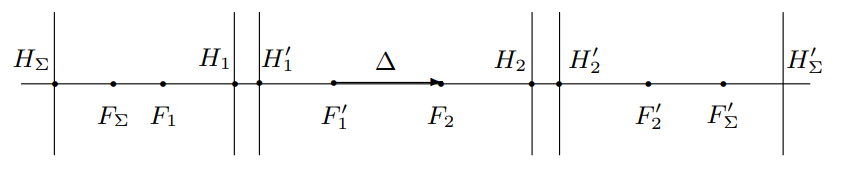
\includegraphics[width=0.8\linewidth]{pics/system_of_lens.png}
        \caption{Сложение центрированных систем}
        \label{}
    \end{figure}


    Конечные уравнения для фокусного расстояния и координат фокальных и главных точек сложной системы:


    \begin{equation}\label{1}
        f_{\sum} = - \frac{f_1 f_2}{\Delta}
    \end{equation}


    \begin{equation}\label{2}
        f'_{\sum } = - \frac{f'_1 f'_2}{\Delta}
    \end{equation}

    \begin{equation}\label{3}
        \Phi = \frac{n}{f_{\sum}} = -\frac{n\Delta}{f_1 f_2}
    \end{equation}



    \textbf{Примеры центрированных оптических систем}
    Оптическая система может не иметь фокальных плоскостей. Такая система называется афокальной или телескопической.
    Она является предельным случаем обычной системы, у которой фокальные плоскости сдвинуты в беконечность.
    Как видно из формул для сложных систем, телескопической становится система из двух обычных систем, если их оптический интервал $\Delta \rightarrow 0$

    Выполнив этот предельный переход в уравнениях, получим формулы для преобразования координат и коэффициенты увеличений телескопической системы:

    \[ \frac{x'}{x} = \frac{\delta x'}{\delta x} = \frac{f_2 f'_2}{f_1 f'_1} \]
    \[ \frac{y'}{y} = \frac{n \alpha}{n' \alpha'} = \frac{f_2}{f'_1} \]
    

    Из выражений выше следует, что в телескопической системе:
    \begin{enumerate}
        \item всякий параллельный пучок света после прохождения через систему остаётся параллельным
        \item продольное, поперечное и угловое увеличения постоянны, то есть не зависят от положения предмета.
    \end{enumerate}

    Оптическая сила телескопической системы, как видно из формулы \ref{3}, равна нулю.



	\section{Экспериментальная установка}
	Схема установки, используемой в работе, показана на рис. \ref{scheme}. Свинцовый коллиматор выделяет узкий почти параллельный пучок $\gamma$-квантов, проходящий через набор поглотителей П и регистрируемый сцинтилляционным счетчиком). Сигналы от счетчика усиливаются и регистрируются пересчетным прибором ПП. Высоковольтный выпрямитель ВВ обеспечивает питание сцинтилляционного счетчика.

При недостаточно хорошей геометрии в результаты опытов могут
вкрасться существенные погрешности. В реальных установках всегда имеется конечная вероятность того, что $\gamma$-квант провзаимодействует в
поглотителе несколько раз до того, как попадет в детектор. Чтобы уменьшить число таких случаев, в данной работе сцинтилляционный счетчик расположен на большом расстоянии от источника $\gamma$-квантов, а поглотители имеют небольшие
размеры. Их следует устанавливать за коллиматорной щелью на некотором расстоянии друг от друга, чтобы испытавшие комптоновское
рассеяние и выбывшие из прямого потока кванты с меньшей вероятностью могли в него вернуться.
	
	\begin{figure}[h!]
		\centering
		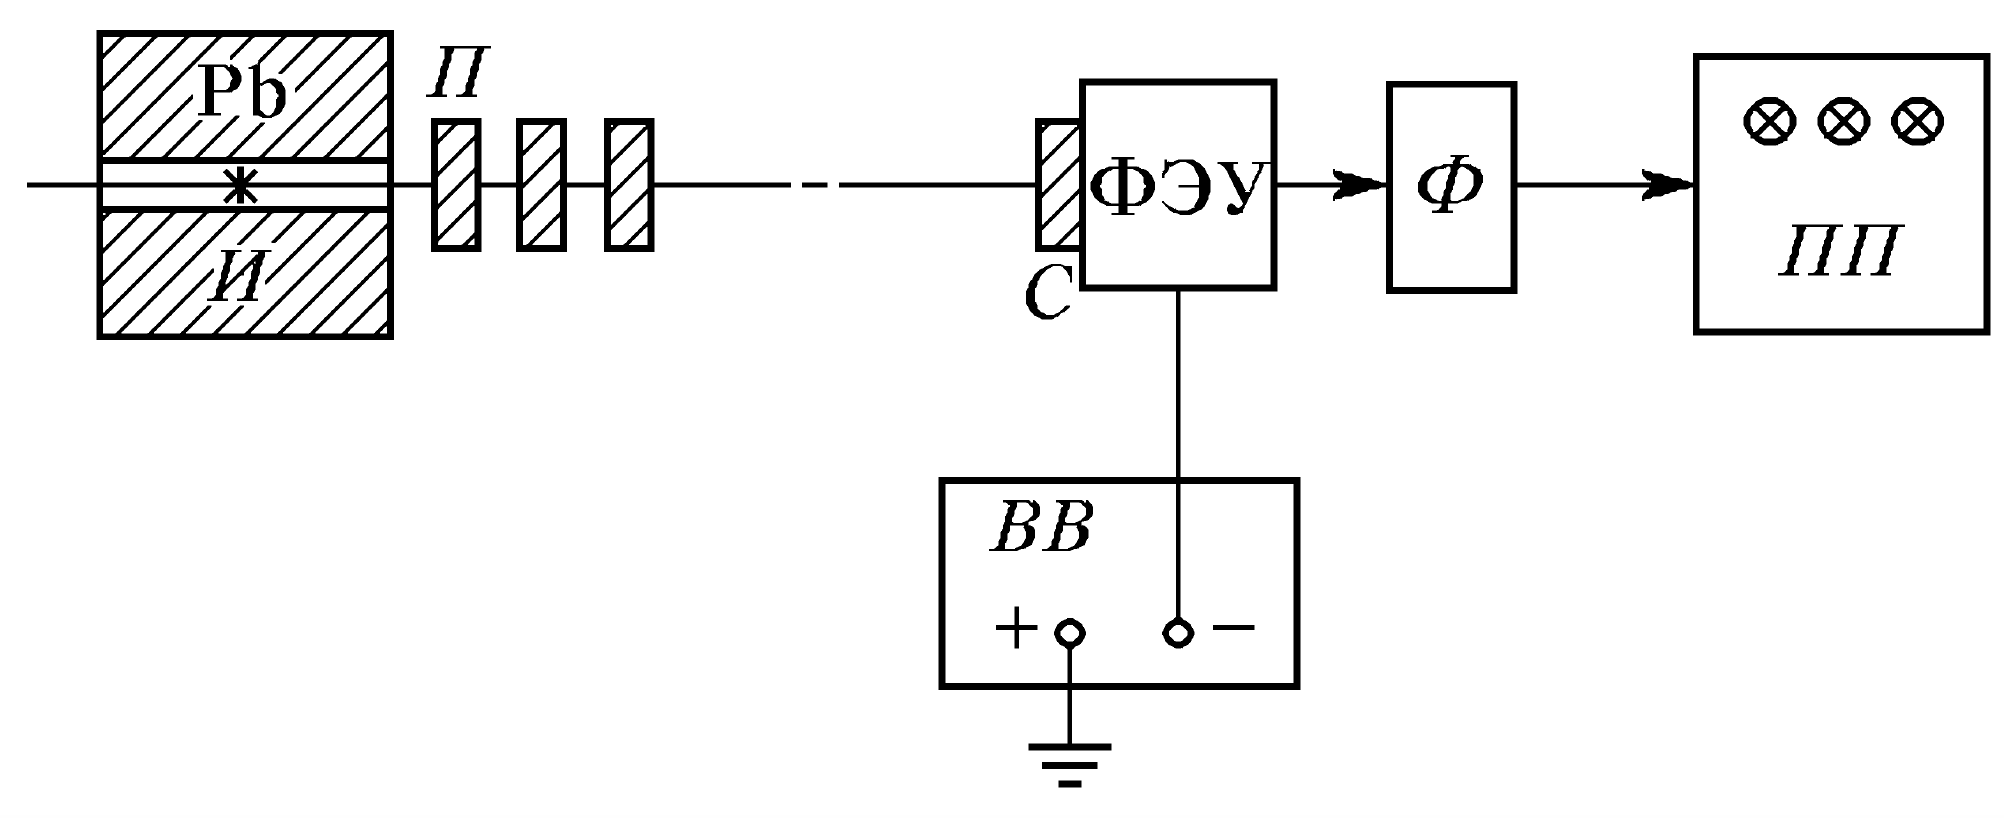
\includegraphics[width=0.8\linewidth]{pics/scheme.png}
		\caption{Блок-схема установки, используемой для измерения коэффициентов ослабления потока $\gamma$-лучей.}
		\label{scheme}
	\end{figure} 

	\begin{figure}[h!]
		\centering
		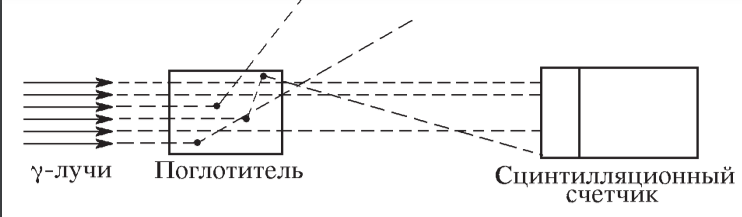
\includegraphics[width=0.8\linewidth]{pics/part_disp.png}
		\caption{Схема рассеяния $\gamma$-квантов в поглотителе.}
		\label{}
	\end{figure}  

	\newpage
	
	\section{Ход работы}

	В условиях эксперимента необходимо учитывать фон, поэтому
	\begin{equation}
		N_0 = n_0 - n_\text{фон}, \ N_i = n_i - n_\text{фон}.
	\end{equation}
	
	\begin{table}[h!]
		\centering
		\begin{tabular}{| c | c | c | c |}
\hline
$$ & $n$ & $t, c$ & $N, \frac{part}{c}$\\
\hline
$N_0$ & $899735$ & $60$ & $14996$\\
\hline
$n_фон$ & $690$ & $60$ & $12$\\
\hline
\end{tabular}

		\caption{: измерения фона и числа частиц $N_0$ без поглотитела}
	\label{tb0}
	\end{table}

	\begin{table}[h!]
		\centering
		\begin{tabular}{| c | c | c | c | c | c | c |}
\hline
$$ & $$ & $$ & $$ & $$ & $$ & $$\\
\hline
$d, mm$ & $N_1$ & $N_2$ & $N_3$ & $t_1, c$ & $t_2, c$ & $t_3, c$\\
\hline
$20$ & $263952$ & $260973$ & $263118$ & $30$ & $30$ & $30$\\
\hline
$39,9$ & $160503$ & $159906$ & $160081$ & $30,51$ & $30,54$ & $30,72$\\
\hline
$59,9$ & $97798$ & $98489$ & $99099$ & $30,56$ & $30,56$ & $30,54$\\
\hline
$80$ & $59773$ & $60059$ & $62402$ & $30,43$ & $30,24$ & $30,63$\\
\hline
$100,1$ & $39806$ & $40409$ & $40142$ & $30,51$ & $30,5$ & $30,52$\\
\hline
$120$ & $25347$ & $25638$ & $25903$ & $30,45$ & $30,45$ & $30,45$\\
\hline
\end{tabular}

		\caption{: измерения числа частиц для алюминия}
	\label{tb0_5}
	\end{table}


	\begin{table}[h!]
		\centering
		\begin{tabular}{| c | c | c | c | c | c | c |}
\hline
$свинец$ & $$ & $$ & $$ & $$ & $$ & $$\\
\hline
$d, mm$ & $N_1$ & $N_2$ & $N_3$ & $t_1, c$ & $t_2, c$ & $t_3, c$\\
\hline
$4,7$ & $455151$ & $432762$ & $433034$ & $60$ & $60$ & $60$\\
\hline
$9,4$ & $213251$ & $211264$ & $213926$ & $60$ & $60$ & $60$\\
\hline
$14,4$ & $57808$ & $60097$ & $60509$ & $30$ & $30$ & $30$\\
\hline
$19$ & $31461$ & $31782$ & $32412$ & $30$ & $30$ & $30$\\
\hline
$24$ & $18439$ & $18414$ & $18550$ & $30,2$ & $30,57$ & $30,56$\\
\hline
\end{tabular}

		\caption{: измерения числа частиц для свинца}
	\label{tb1_5}
	\end{table}

	

	\begin{table}[h!]
		\centering
		\begin{tabular}{| c | c | c | c | c | c | c | c | c |}
\hline
$железо$ & $$ & $$ & $$ & $$ & $$ & $$ & $$ & $$\\
\hline
$d, mm$ & $N_1$ & $N_2$ & $N_3$ & $<N>$ & $N$ & $t_1, c$ & $t_2, c$ & $t_3, c$\\
\hline
$10$ & $115277$ & $113948$ & $114488$ & $114571$ & $7374$ & $15,42$ & $15,54$ & $15,65$\\
\hline
$20,1$ & $54906$ & $54438$ & $55587$ & $54977$ & $3549$ & $15,51$ & $15,55$ & $15,41$\\
\hline
$30,2$ & $27951$ & $28301$ & $28747$ & $28333$ & $1819$ & $15,45$ & $15,56$ & $15,71$\\
\hline
$40,3$ & $15106$ & $14870$ & $15330$ & $15102$ & $980$ & $15,44$ & $15,29$ & $15,49$\\
\hline
$50,4$ & $8412$ & $8315$ & $8274$ & $8334$ & $537$ & $15,54$ & $15,41$ & $15,6$\\
\hline
$60,4$ & $4564$ & $4560$ & $4553$ & $4559$ & $294$ & $15,52$ & $15,53$ & $15,45$\\
\hline
\end{tabular}

		\caption{: измерения числа частиц для железа}
	\label{tb2_5}
	\end{table}

	\newpage
	\section{Обработка результатов}

	\textbf{Погрешности}
	При повторном проведении опыта измренения количества частиц для фиксирванной длины замечаем, что измеренная величина отличается не более чем на 3\% от среднечего значения. 
	На самом деле среднее значение отклонения от среднего $\sim$ 0,5 $\div$ 1,5 \%. Но беру с запасом веррхнюю границу. Значит, 
	
	\[ \frac{\sigma_N}{N} \approx \frac{\sigma_{N_{0}}}{N_{0}} = 0,03 \]

	\[	\sigma_{\ln\left(\frac{N_0}{N}\right)} = \frac{1}{\frac{N_0}{N}} \sigma_{N_0/N} = \frac{1}{\frac{N_0}{N}} \cdot \frac{N_0}{N} \cdot \sqrt{\left(\frac{\sigma_{N_0}}{N_0}\right)^2+\left(\frac{\sigma_{N}}{N}\right)^2} \]

	\[  \sigma_{\ln\left(\frac{N_0}{N}\right)} \approx = 0,042 \]


	Погрешность измерения длины поглотителя - это просто погрешность штангециркуля, т.к. каждый измерения происходили после каждого добавления нового слоя.
	Таким образом, $\sigma_d = 0,01 см$
		
	
	Обрабтаем полученные во время работы данные:

	\begin{itemize}
		\item определим среднее число частиц 3-х измерений для фиксированной длины
		\item определим число частиц, детектируемое за 1 секунду
		\item учтем рассчитанную погрешность
		\item построим графики для свинца, железа, алюминия
	\end{itemize}

	\begin{table}[h!]
		\centering
		\begin{tabular}{| c | c | c | c | c |}
\hline
$U, mV$ & $T_{room}, K$ & $T, K$ & $T_{br}, K$ & $ \sigma_{T}, K$\\
\hline
$39920$ & $298$ & $973,66$ & $1000$ & $ 28 $\\
\hline
\end{tabular}

		\caption{: обработанные данные для алюминия}
	\label{tb1}
	\end{table}

	\begin{table}[h!]
		\centering
		\begin{tabular}{| c | c | c | c | c |}
\hline
$\theta,^{\circ}$ & $U(I)$ & $V_{ФЭ}$ & $\sigma_{U(I)}$ & $\sigma_{V_{ФЭ}}$\\
\hline
$2404$ & $0,036$ & $0,302$ & $0,0004$ & $0,003$\\
\hline
$$ & $0,032$ & $0,262$ & $0,0004$ & $0,003$\\
\hline
$$ & $0,027$ & $0,202$ & $0,0004$ & $0,003$\\
\hline
$$ & $0,02$ & $0,121$ & $0,0004$ & $0,003$\\
\hline
$$ & $0,016$ & $0,039$ & $0,0004$ & $0,003$\\
\hline
$$ & $0,009$ & $-0,062$ & $0,0004$ & $0,003$\\
\hline
$$ & $0,006$ & $-0,162$ & $0,0004$ & $0,003$\\
\hline
$$ & $0$ & $-0,303$ & $0,0004$ & $0,003$\\
\hline
\end{tabular}

		\caption{: обработанные данные для свинца}
	\label{tb2}
	\end{table}

	\begin{table}[h!]
		\centering
		\begin{tabular}{| c | c |}
\hline
$ln(T_{term})$ & $ln(P)$\\
\hline
$6,82$ & $2,43$\\
\hline
$6,96$ & $2,88$\\
\hline
$7,05$ & $3,42$\\
\hline
$7,15$ & $3,73$\\
\hline
$7,22$ & $3,98$\\
\hline
$7,31$ & $4,25$\\
\hline
$7,38$ & $4,48$\\
\hline
$7,4$ & $4,72$\\
\hline
$7,48$ & $4,88$\\
\hline
$7,51$ & $5,1$\\
\hline
$7,55$ & $5,29$\\
\hline
\end{tabular}

		\caption{: обработанные данные для железа}
	\label{tb3}
	\end{table}	
	
	

	\begin{table}[h!]
		\centering
		\begin{tabular}{| c | c | c | c |}
\hline
$d, cm$ & $ln(N_0/N)$ & $\sigma_{d}, см$ & $\sigma_{ln(N_0/N)}$\\
\hline
$2$ & $0,54$ & $0,01$ & $0,042$\\
\hline
$3,99$ & $1,05$ & $0,01$ & $0,042$\\
\hline
$5,99$ & $1,54$ & $0,01$ & $0,042$\\
\hline
$8$ & $2,02$ & $0,01$ & $0,042$\\
\hline
$10,01$ & $2,44$ & $0,01$ & $0,042$\\
\hline
$12$ & $2,89$ & $0,01$ & $0,042$\\
\hline
\end{tabular}

		\caption{: данные для графика, алюминий}
	\label{tb4}
	\end{table}

	\begin{table}[h!]
		\centering
		\begin{tabular}{| c | c | c | c | c |}
\hline
$\theta,^{\circ}$ & $U(I)$ & $V_{ФЭ}$ & $\sigma_{U(I)}$ & $\sigma_{V_{ФЭ}}$\\
\hline
$2500$ & $0,514$ & $7$ & $0,005$ & $0,07$\\
\hline
$$ & $0,5$ & $5,999$ & $0,005$ & $0,07$\\
\hline
$$ & $0,48$ & $5$ & $0,005$ & $0,07$\\
\hline
$$ & $0,472$ & $4,495$ & $0,005$ & $0,07$\\
\hline
$$ & $0,456$ & $3,999$ & $0,005$ & $0,07$\\
\hline
$$ & $0,434$ & $3,505$ & $0,005$ & $0,07$\\
\hline
$$ & $0,406$ & $2,998$ & $0,005$ & $0,07$\\
\hline
$$ & $0,36$ & $2,5$ & $0,005$ & $0,07$\\
\hline
$$ & $0,273$ & $1,998$ & $0,005$ & $0,07$\\
\hline
$$ & $0,165$ & $1,49$ & $0,005$ & $0,07$\\
\hline
$$ & $0,13$ & $1,25$ & $0,005$ & $0,07$\\
\hline
$$ & $0,087$ & $1,002$ & $0,005$ & $0,07$\\
\hline
$$ & $0,06$ & $0,75$ & $0,005$ & $0,07$\\
\hline
$$ & $0,038$ & $0,5$ & $0,005$ & $0,07$\\
\hline
$$ & $0,021$ & $0,249$ & $0,005$ & $0,07$\\
\hline
$$ & $0,013$ & $0,1$ & $0,005$ & $0,07$\\
\hline
$$ & $0,008$ & $0,009$ & $0,005$ & $0,07$\\
\hline
$$ & $0,006$ & $-0,05$ & $0,005$ & $0,07$\\
\hline
$$ & $0,003$ & $-0,1$ & $0,005$ & $0,07$\\
\hline
$$ & $0,002$ & $-0,15$ & $0,005$ & $0,07$\\
\hline
$$ & $0,001$ & $-0,2$ & $0,005$ & $0,07$\\
\hline
$$ & $0$ & $-0,249$ & $0,005$ & $0,07$\\
\hline
\end{tabular}

		\caption{: данные для графика, свинец}
	\label{tb5}
	\end{table}

	\begin{table}[h!]
		\centering
		\begin{tabular}{| c | c | c | c | c |}
\hline
$\theta, ^{\circ}$ & $U(I)$ & $V_{ФЭ}$ & $\sigma_{U(I)}$ & $\sigma_{V_{ФЭ}}$\\
\hline
$2162$ & $0,49$ & $7,46$ & $0,005$ & $0,07$\\
\hline
$$ & $0,487$ & $7,377$ & $0,005$ & $0,07$\\
\hline
$$ & $0,481$ & $7,003$ & $0,005$ & $0,07$\\
\hline
$$ & $0,47$ & $6,504$ & $0,005$ & $0,07$\\
\hline
$$ & $0,462$ & $6$ & $0,005$ & $0,07$\\
\hline
$$ & $0,45$ & $5,508$ & $0,005$ & $0,07$\\
\hline
$$ & $0,43$ & $5,005$ & $0,005$ & $0,07$\\
\hline
$$ & $0,41$ & $4,5$ & $0,005$ & $0,07$\\
\hline
$$ & $0,383$ & $4,003$ & $0,005$ & $0,07$\\
\hline
$$ & $0,343$ & $3,5$ & $0,005$ & $0,07$\\
\hline
$$ & $0,281$ & $3$ & $0,005$ & $0,07$\\
\hline
$$ & $0,215$ & $2,503$ & $0,005$ & $0,07$\\
\hline
$$ & $0,156$ & $2,001$ & $0,005$ & $0,07$\\
\hline
$$ & $0,127$ & $1,75$ & $0,005$ & $0,07$\\
\hline
$$ & $0,103$ & $1,5$ & $0,005$ & $0,07$\\
\hline
$$ & $0,084$ & $1,25$ & $0,005$ & $0,07$\\
\hline
$$ & $0,075$ & $1,125$ & $0,005$ & $0,07$\\
\hline
$$ & $0,066$ & $1$ & $0,005$ & $0,07$\\
\hline
$$ & $0,059$ & $0,9$ & $0,005$ & $0,07$\\
\hline
$$ & $0,051$ & $0,8$ & $0,005$ & $0,07$\\
\hline
$$ & $0,045$ & $0,7$ & $0,005$ & $0,07$\\
\hline
$$ & $0,033$ & $0,6$ & $0,005$ & $0,07$\\
\hline
$$ & $0,031$ & $0,5$ & $0,005$ & $0,07$\\
\hline
$$ & $0,027$ & $0,4$ & $0,005$ & $0,07$\\
\hline
$$ & $0,017$ & $0,2$ & $0,005$ & $0,07$\\
\hline
$$ & $0,013$ & $0,1$ & $0,005$ & $0,07$\\
\hline
$$ & $0,009$ & $0,01$ & $0,005$ & $0,07$\\
\hline
$$ & $0,005$ & $-0,1$ & $0,005$ & $0,07$\\
\hline
$$ & $0,002$ & $-0,2$ & $0,005$ & $0,07$\\
\hline
$$ & $0$ & $-0,3$ & $0,005$ & $0,07$\\
\hline
\end{tabular}

		\caption{: данные для графика, железо}
	\label{tb6}
	\end{table}

	Учтем погрешность МНК:

	\[ \sigma_{\mu} = \dfrac{1}{\sqrt{n}}\sqrt{\dfrac{\langle y^2 \rangle - \langle y \rangle^2}{\langle x^2 \rangle - \langle x \rangle^2} - \mu^{2}} \]

	Из построенных графиков по МНК получаем, что:

	\begin{table}[h!]
		\centering
		\begin{tabular}{| c | c | c |}
\hline
$образец$ & $\mu , 1/c$ & $\sigma_{\mu}, 1/c$\\
\hline
$Al$ & $0,234$ & $0,0038$\\
\hline
$Pb$ & $1,29$ & $0,0536$\\
\hline
$Fe$ & $0,641$ & $0,0618$\\
\hline
\end{tabular}

		\caption{: результаты}
	\label{tb6}
	\end{table}

	Из таблицы 4 приложения V получаем соответствующую среднюю энерги $\gamma$ - лучей, испускаемых истчочником:

	\begin{itemize}
		\item $\mu_{Al} = 0,234 \pm 0,0038 \Rightarrow E_{\gamma} \approx 0,4 \div 0,5 \text{ МЭв} $
		\item $\mu_{Pb} = 1,23 \pm 0,053 \Rightarrow E_{\gamma} \approx 0,6 \text{ МЭв} $
		\item $\mu_{Fe} = 0,234 \pm 0,0038 \rightarrow E_{\gamma} \approx 0,4 \div 0,5 \text{ МЭв} $
	\end{itemize}

	\begin{figure}[h!]
		\centering
		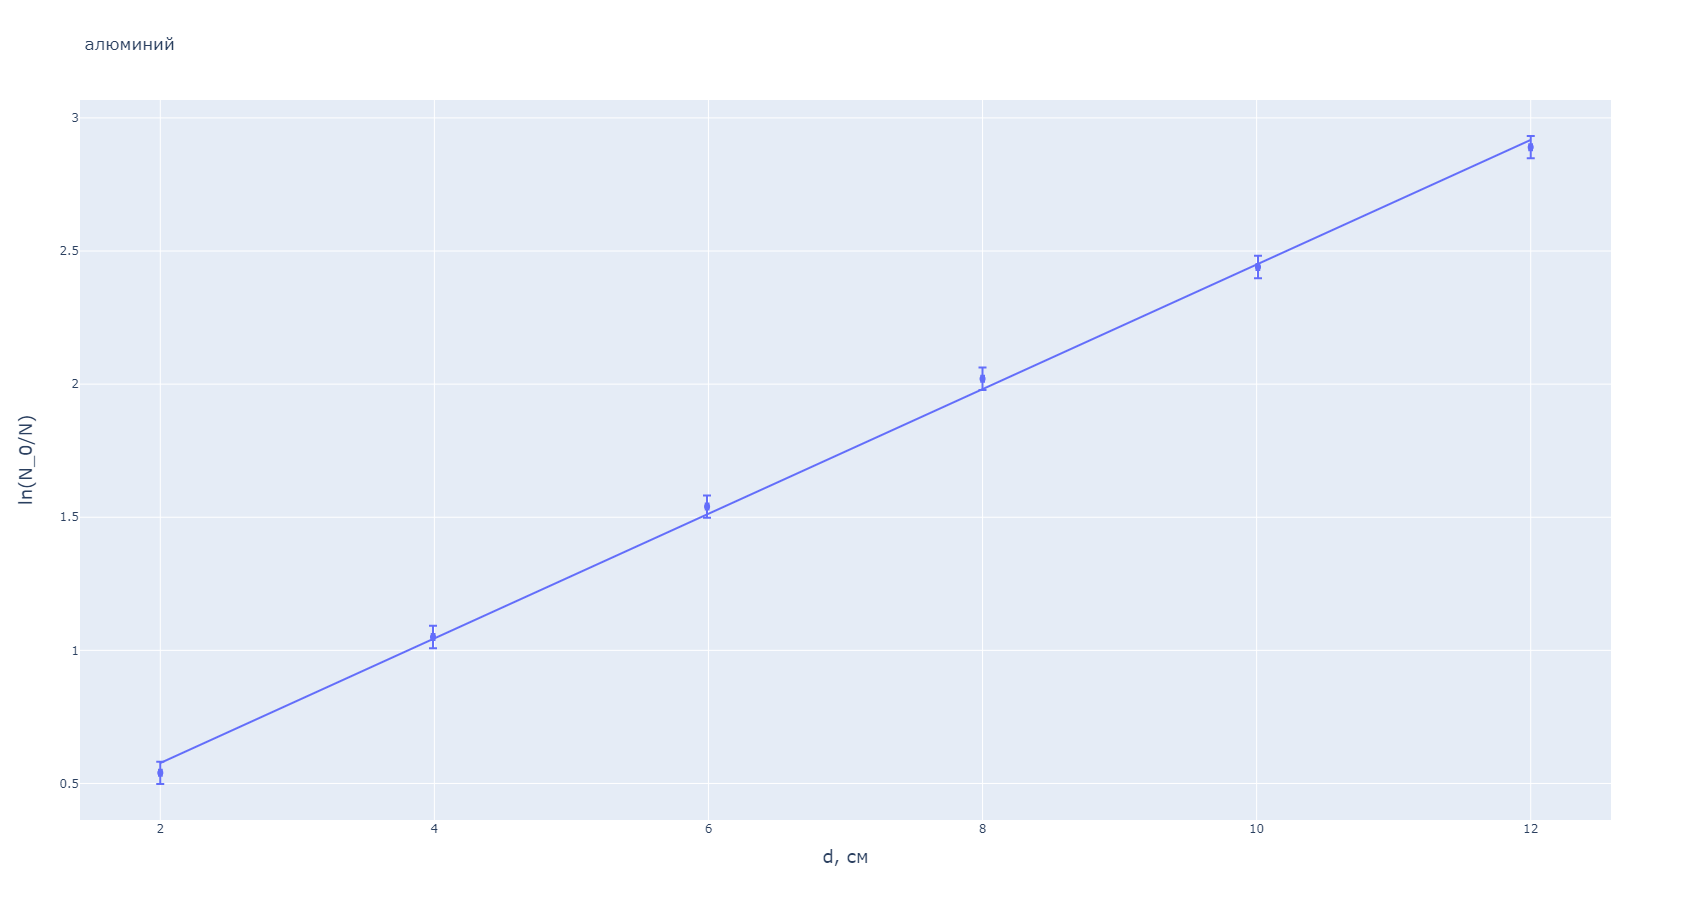
\includegraphics[width=1.0\linewidth]{pics/al.png}
		\caption{ : зависимость для алюминия}
		\label{al}
	\end{figure}

	\begin{figure}[h!]
		\centering
		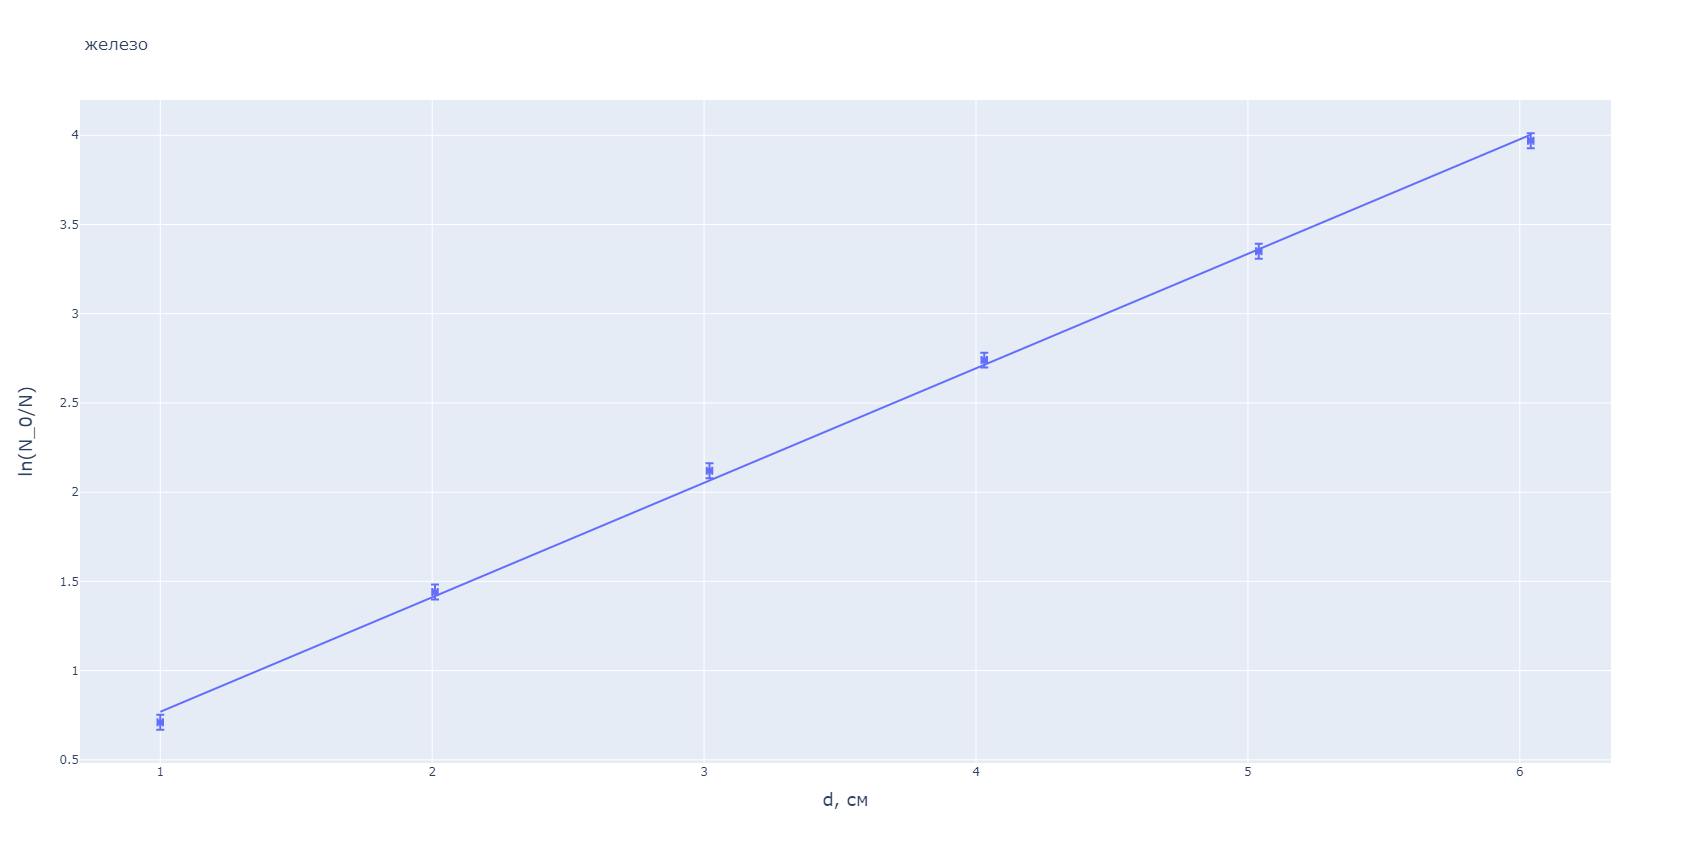
\includegraphics[width=1.0\linewidth]{pics/fr.png}
		\caption{ : зависимость для железа}
		\label{fr}
	\end{figure}

	\begin{figure}[h!]
		\centering
		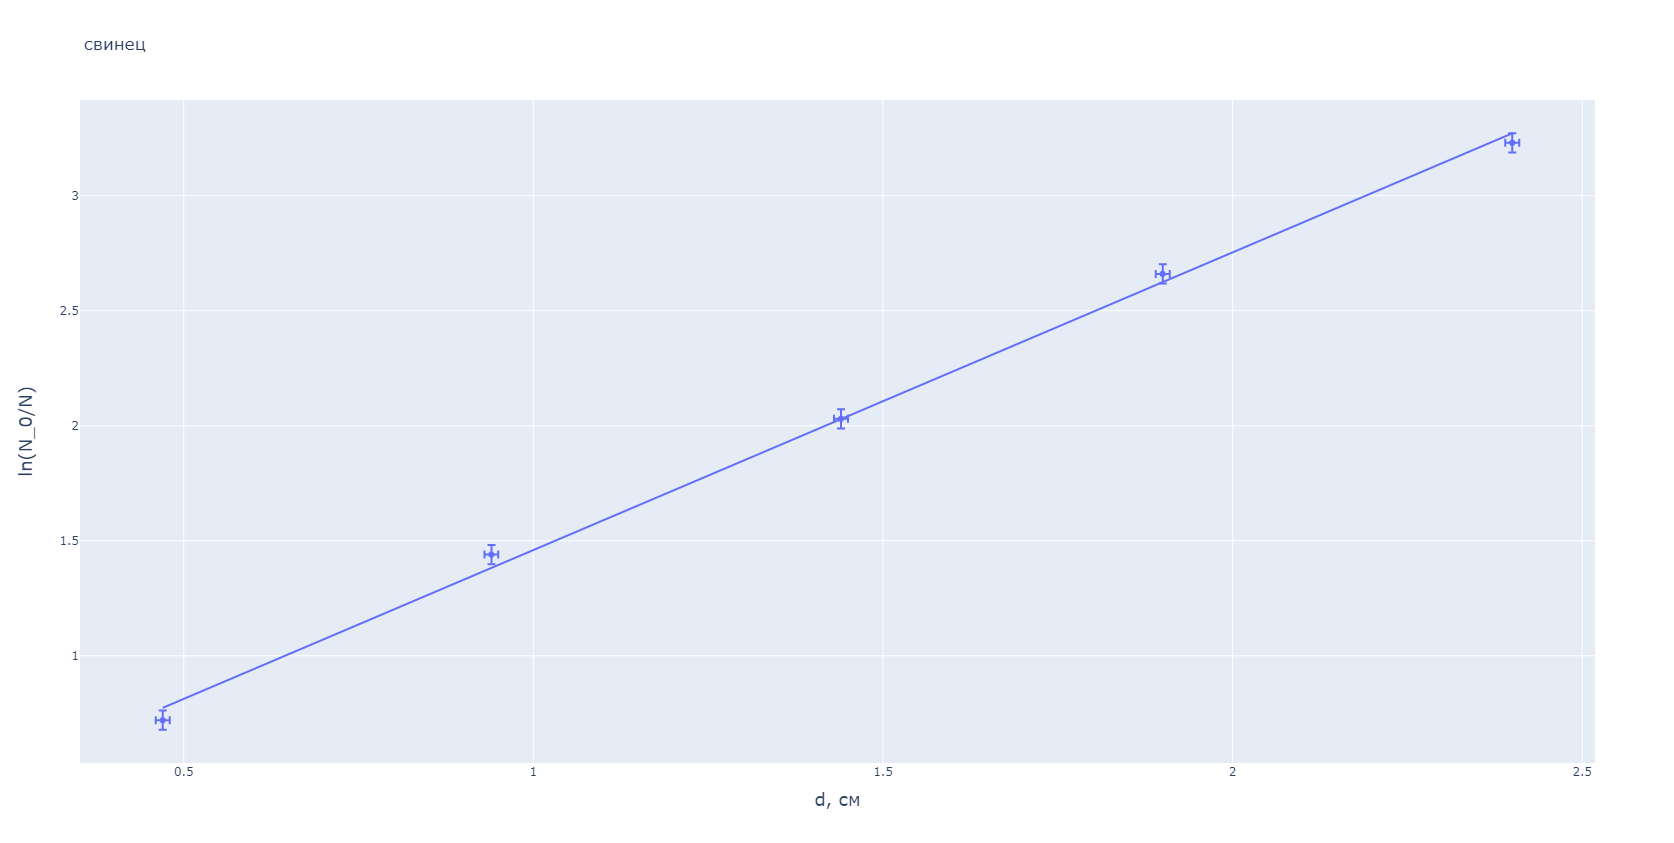
\includegraphics[width=1.0\linewidth]{pics/pb.png}
		\caption{ : зависимость для свинца}
		\label{pb}
	\end{figure}

	\newpage

	\section{Вывод}
	В настоящей лабораторной работе с помощью сцинтилляционного счетчика были измерены линейные коэффициенты ослабления $\mu$ потока $\gamma$-лучей в свинце, железе, алюминии. 
	Среднюю энергию излучения, испускаемого источником, определили по справочной таблице, приведенной в приложении лабораторного практикума по общей физике.

	Приведу результаты еще раз дам небольшой анализ.

	\begin{itemize}
		\item $\mu_{Al} = 0,234 \pm 0,0038 \Rightarrow E_{\gamma} \approx 0,4 \div 0,5 \text{ МЭв} $
		\item $\mu_{Pb} = 1,23 \pm 0,053 \Rightarrow E_{\gamma} \approx 0,6 \text{ МЭв} $
		\item $\mu_{Fe} = 0,234 \pm 0,0038 \rightarrow E_{\gamma} \approx 0,4 \div 0,5 \text{ МЭв} $
	\end{itemize}

	\begin{enumerate}
		\item значения линейных коэффициентов, а также погрешности получились адекватного порядка.
		\item средняя энергия испускаемых квантов получилась \textbf{для каждого вещества} приблизительно порядка $\approx 0,5 \text{ МЭв}$
	\end{enumerate}

	Учитывая два пункта, приведенных выше, можно считать, что эксперимент проведён успешно и полученные значения в пределах погрешности соответствуют реальным значениям. 

\end{document}





